
\chapter{System Parameterization \& Weight Profile Synthesis}
\label{sec:param}

Every dimension of the data frame $\mathbf{X} \in \mathbb{C}^{M \times N}$ and of the weight matrix $\mathbf{W} \in \mathbb{C}^{K \times R}$ is fixed by an explicit operational requirement --- the array hardware, the correlator's framing contract, the fixed-point arithmetic budget, or the spectral structure of the interference being detected --- rather than left as a free tuning parameter. This section derives each parameter from its governing constraint (Section~\ref{sec:param:tradeoffs}), then constructs the weight profiles themselves: the target matched filter synthesized from the broadcast standard's pilot carrier (Section~\ref{sec:param:target}) and the displaced reference profiles that furnish the background estimate (Section~\ref{sec:param:refs}). A recurring theme, developed fully in Chapter~\ref{sec:impl}, is that the entire datapath downstream of these weights is exact integer arithmetic; several parameter choices below exist precisely to make that exactness possible.

\section{Architectural Trade-Offs \& Parameter Justifications}
\label{sec:param:tradeoffs}

\begin{enumerate}
    \item \textbf{Telescope Feed Count ($M = 2048$):} The spatial dimension $M = 2^{11} = 2048$ is strictly hardware-defined, corresponding to the total number of independent spatial inputs processed by the telescope array: four cylindrical reflectors, each instrumented with 256 dual-polarization feeds, giving 1024 antennas and $M = 2048$ analog chains \cite{amiri2022chime}. The detector does not require per-feed phase calibration: as developed in Section~\ref{sec:pipeline:noncoherent}, all cross-feed combining is non-coherent by design.  The analytic null model initially treats the inputs as independent noise looks, but this is an approximation rather than a hardware identity; common sky signal, receiver coupling, and shared gain structure can reduce the effective degrees of freedom.  The empirical null calibration therefore remains authoritative, and a release-quality calibration reports the effective-width inflation relative to the independent-feed model.

    \item \textbf{Correlator Frame Synchronization ($N = 16384$):} The temporal frame length is fixed at $N = 2^{14} = 16384$ complex samples, the design value of the upgraded correlator engine's integration frame contract; at the receiver coarse-channel rate $f_s = 390.625$~kHz (the 400~MHz observing bandwidth divided into 1024 channelizer channels \cite{amiri2022chime}) this corresponds to a frame cadence of $41.94$~ms. Matching the correlator frame one-to-one is a structural decision, not a convenience: the detector's product is a per-frame rejection flag applied to the visibility integration of \emph{the same samples}. Any mismatch between detection frames and correlator frames would force one of two failure modes --- interpolating flags across partially overlapping integrations (contaminating clean integrations with flagged fractions, and vice versa), or buffering and re-framing the baseband (adding latency and a second framing contract to keep synchronized). The contract that eliminates both is that a decision must span an \emph{integer} number of correlator integrations: a flag either applies to an integration or it does not, with no partial-frame semantics. The target upgraded interface is the $1{:}1$ case. A receiver whose visibility integration is shorter than its detector frame realizes an $n{:}1$ case, which is equally free of partial-frame semantics but coarsens the excision quantum by $n$ --- a real cost against intermittent interference, and the reason $N$ is specified as an interface value rather than as a universal constant. The published correlator integrates visibilities over 12{,}288 channelized samples ($\approx31$~ms) \cite{amiri2022chime}, whereas $N = 16384$ is the upgraded-engine design used and benchmarked here. Chapter~\ref{sec:deployment} therefore treats frame alignment as an integration acceptance gate, not as an already demonstrated live property; nothing in the detector construction depends on the specific value beyond the power-of-two tiling discussed next.

    \item \textbf{Exact-Arithmetic and Geometric Weight Length ($K = 128$):} The tap length is set by exact-arithmetic and geometric constraints rather than by a sensitivity optimum, and it is \emph{derived} rather than chosen: $K$ is the power of two whose sub-frame rate $f_s/K$ meets the analysis-window requirement set by the measured transmitter population of Section~\ref{sec:dtv:environment}, subject to the fixed-point ceiling of item (c). At CHIME's $f_s = 390.625$~kHz that evaluates to $K = 2^7 = 128$; the same requirement on a receiver whose coarse raster is half as wide gives $K = 64$, since what the population fixes is the window \emph{width in frequency}, not the tap count. Sensitivity does not constrain this parameter: because the coherent spectral integration of Section~\ref{sec:pipeline:coherent} restores coherence across the full frame regardless of how the frame is partitioned (the product $KL = N$ is fixed), the detector's deflection is governed by $N$ to first order; $K$ selects only the sub-frame geometry --- where the boundary falls between the matched-filter projection and the cross-window transform. Within that freedom, $K = 128$ is pinned by four requirements:
    \begin{enumerate}
        \item \emph{Exact frame tiling.} $K$ must divide $N$ exactly with both factors powers of two, giving $L = N/K = 128$ complete sub-frames with no residual samples and radix-2-friendly transform lengths at every stage.
        \item \emph{Fine-span coverage of the measured offset population.} The sub-frame rate $f_s / K \approx 3.052$~kHz sets the unambiguous span of the fine spectral axis at $\pm f_s/(2K) \approx \pm 1.526$~kHz. Because the synthesized tone absorbs each pilot's nominal channelization offset exactly (Section~\ref{sec:param:target}), this span need only cover the \emph{residual} offsets that actually occur --- and that requirement is empirical, fixed by the census of Section~\ref{sec:dtv:environment}: the disciplined primary core, the undisciplined secondary skirt, and the ${\approx}\pm 1$~kHz aircraft-Doppler envelope on scattered components. $K = 128$ covers that population with margin, and the survey-measured anchors certify the sizing on archived telescope data: the largest measured residual, $-1.37$~kHz on channel 32, sits at $90\%$ of the span edge --- inside $K = 128$'s span, \emph{outside} the $\pm 0.763$~kHz span of the next radix-2 step $K = 256$, which would have clipped a measured primary outright (and which item (c)'s conservative bit bound excludes independently). The step down closes the bracket from the other side: $K = 64$ widens the span to $\pm 3.05$~kHz, but the reference displacement is $\pm 2$ bins \emph{of the $K$-tap grid} --- $\pm 2 f_s/K$ in frequency --- so halving $K$ doubles the references' distance to $\pm 12.2$~kHz, quadrupling the surviving curvature term of item 4's slope cancellation and moving the background samples away from the locally smooth neighborhood the ratio statistic requires. The radix-2 bracket around $K = 128$ is thus closed on both sides by measurement rather than preference: $256$ clips the population the census maps, $64$ degrades the background estimate the ratio needs, and $128$ covers the one while preserving the other. Both disqualifications are statements at CHIME's $f_s$ rather than about tap counts in isolation: on a receiver whose coarse raster is half as wide, $K = 64$ reproduces exactly the span and reference displacement in frequency that $K = 128$ realizes here, per the derivation above. One honest boundary of the coverage claim is visible in Figure~\ref{fig:census:psd}: on the most crowded channels a minority of sidelobe structure falls \emph{outside} the span (channel 33's second primary at ${\approx}{-}4$~kHz is the clearest case), and no radix-2 value covers it without ruining the reference geometry --- $K = 32$ would reach it at the price of references $\pm 24$~kHz out. The window is sized to capture the \emph{dominant} emitter on every channel; out-of-span structure aliases across the fine axis and is handled where it belongs, by the decision architecture (bulk, census exclusions, and the rank's contamination immunity, Section~\ref{sec:pipeline:decision}) rather than by the window. A final constraint completes the choice: $K$ is a single band-wide constant, not a per-channel one. A per-channel tap length would fragment the kernel geometry, the weight-bank contract, the transform family, and the verification corpus into as many variants as channels --- operationally undesirable for the single-geometry implementation evaluated here --- so one value must serve the whole monitored band, and it is selected for the majority of channels with the weight placed on those whose potential science return is largest. That weighting is visible in the outcome: the channels $K = 128$ serves completely include every channel that is threshold-feasible under the current conditional forecast of Section~\ref{sec:bao:thresholds}, and the imperfectly-served minority structure lies on channels whose verdicts do not hinge on it.
        \item \emph{Fixed-point bit-growth closure.} The exact integer datapath requires the complete dot product to fit fixed-width accumulators with no possibility of overflow. With 4-bit signed components, samples lie in $[-8, 7]$ and quantized weight components in $[-7, 7]$ (the receiver's own quantizer is in fact 15-level mid-tread, emitting only $[-7, 7]$ \cite{menaparra2018}; the datapath bound conservatively admits the full two's-complement range), so one complex-product component is bounded by $|x_r w_r| + |x_i w_i| \le 8 \cdot 7 + 8 \cdot 7 = 112$; accumulating $K = 128$ taps bounds the completed dot-product component at $128 \times 112 = 14336 < 2^{14}$. Equivalently: a $4{\times}4$-bit product pair contributes $4 + 4 + 1 = 9$ bits, and $\log_2 K$ accumulation guard bits bring the total to $9 + \log_2 K$ --- exactly 16 signed bits at $K = 128$, the natural register width, with headroom. Each downstream stage carries its own bound derived from the same quantity: the coarse squared magnitude $2(128K)^2$ against the 32-bit accumulator, and the transform's per-stage growth against the same width. In the implemented kernel these are not prose but \texttt{static\_assert}s evaluated per geometry, so the build --- not a reader --- answers whether a given $K$ closes. The signed-32-bit squared-magnitude bound is the binding one, admitting $K \le 292$ under the true weight range and $K \le 128$ under the conservative bound used here; the guard-bit count is asserted equal to $\log_2 K$ so it cannot silently desynchronize from the window length. The 4-bit grid itself is not the detector's choice but the receiver's: the F-engine rounds its channelized output to packed $4{+}4$-bit complex samples, applying per-channel complex gains beforehand to load that grid optimally \cite{amiri2022chime,menaparra2018}, and the detector adopts the same grid for its weight coefficients so that samples and weights share a single packed integer datapath.
        \item \emph{Kernel geometry.} On the benchmark GPU, the packed \texttt{int4} dot product consumes two complex samples per fused instruction, so $K$ presents $K/2$ packed tap-pairs. In the \emph{staged} projection entry points these are distributed across the block, and $K = 128$ against a 64-thread block gives exactly one pair per thread with no inactive lanes. The implemented \emph{fused} kernel distributes the window axis instead (Section~\ref{sec:impl:fused}): each thread owns whole windows and iterates the $K/2$ tap-pairs serially, so its block geometry is constrained by the window count $L$ rather than by $K$, and $K$ enters only as an inner trip count. This is the weakest of the four constraints and the only one that does not bind the fused form.
    \end{enumerate}
    These four constraints concern the exactness and efficiency of the downstream arithmetic rather than detection statistics: sensitivity is set by the frame length and the coherent transform, while $K$ is selected so that the implementation can be verified at the bit level.

    \item \textbf{Symmetric Reference Count ($N_{\text{ref}} = 2$) and Slope Cancellation:} The number of reference profiles is fixed at $N_{\text{ref}} = 2$, placed symmetrically about the target. Three independent justifications converge on this choice, and the alternatives they exclude are stated at the end of this item.  The cancellation argument is local: it assumes that the two references sample the same sufficiently smooth response in a coordinate for which the placement is symmetric.  A narrow instrumental line, an edge, or any other non-smooth or asymmetric feature inside the span is not cancelled by symmetry and must be handled empirically.

    First, \emph{baseline cancellation}. In astrophysical and instrumental RF environments the background power spectral density across nearby bins is smooth but not flat; expanding it about the target bin as $P_{\text{bg}}(k) = P_0 + \alpha_1 k + \alpha_2 k^2 + \alpha_3 k^3 + \cdots$, a single reference displaced by $\Delta k$ estimates $P_0$ with a first-order error $\alpha_1 \Delta k$. A symmetric pair at $\pm \Delta k$, averaged, cancels \emph{every odd-order term identically}:
    \begin{equation}
    \frac{1}{2}\left( P_{\text{bg}}(+\Delta k) + P_{\text{bg}}(-\Delta k) \right) = P_0 + \alpha_2 \Delta k^2 + \alpha_4 \Delta k^4 + \cdots,
    \end{equation}
    leaving a leading smooth residual of second order, $\alpha_2 \Delta k^2 = 4\alpha_2$ at the implemented $\Delta k = 2$.  For a locally smooth response sampled symmetrically, linear tilt and all other odd Taylor terms cancel algebraically; even-order curvature remains.  Discrete or asymmetric structure is outside this Taylor model and is diagnosed from the recorded spectra rather than claimed to cancel.

    Second, \emph{statistical sufficiency}. The reference estimate enters the test statistic's denominator with $\beta N_{\text{ref}} M$ degrees of freedom (Section~\ref{sec:pipeline:decision}); at $M = 2048$ the two-reference denominator already carries $8192$ degrees of freedom, for a relative standard deviation of $\sqrt{2/8192} \approx 1.6\%$. Adding a third reference would narrow the idealized null from $2.71\%$ to $2.55\%$ --- a $6\%$ improvement --- at the cost of a $33\%$ increase in projection compute and weight-bank storage, moreover, it would provide no practical improvement in the measured operating regime: the \emph{measured} null is inflated several-fold above the i.i.d.\ model by receiver systematics (Section~\ref{sec:pipeline:decision}), so idealized-variance refinements are not the binding constraint. $N_{\text{ref}} = 2$ is therefore the minimum count providing exact odd-order cancellation under the stated local-smoothness model; additional references yield statistically negligible improvement at material computational cost.

    Third, \emph{the reference-window sizing law}. How many reference cells a CFAR detector should carry is a solved problem in the radar literature: the penalty for estimating one's own threshold (the \emph{CFAR loss}) falls with reference count along a universal curve, and the window is sized at that curve's knee \cite{finn1968,gandhi1988}; the same law governs training-sample counts in adaptive detection through the Reed--Mallett--Brennan rule \cite{reed1974}. Applied to this geometry the curve has a closed form: the idealized null width of the ratio scales as $\sqrt{1 + 1/N_{\text{ref}}}$ relative to a perfect (infinite-reference) denominator --- a detection-floor penalty of $0.9$~dB at $N_{\text{ref}} = 2$, $0.6$ at three, $0.5$ at four, with $0.5$~dB unrecoverable at \emph{any} count because it belongs to the single target column, whose own fluctuation no reference reduces. The knee sits at two-to-three, and the reason it sits so low is the feed axis: a radar reference cell is a single look carrying $\beta = 2$ degrees of freedom, so classic windows need $16$--$32$ cells, while each reference here is a full weight column pooled over $M = 2048$ inputs --- $\beta M = 4096$ degrees of freedom per reference. The feed count does for this detector what the cell count does for radar, and $N_{\text{ref}} = 2$ sits where a radar designer's several-thousand-cell window would. Past the knee, the remaining idealized fraction of a decibel is not real in any case: the measured nulls are inflated $14$--$19\times$ above the i.i.d.\ model by systematics (Section~\ref{sec:pipeline:decision}), so the operating width is carried by the contaminated tail, not by denominator degrees of freedom.

    Three alternatives from the CFAR family were weighed and declined, each for a stated reason. \emph{More references of the same kind} purchase the saturating curve above: $+33\%$ of the dominant projection cost per added column for at most $0.4$~dB of idealized floor that the measured null structure erases. \emph{Higher-order cancellation designs} --- pairs at $\pm 2$ and $\pm 4$ bins combined with Richardson weights $(\tfrac{4}{3}, -\tfrac{1}{3})$, which null the quadratic term exactly and leave a fourth-order residual --- pay the Savitzky--Golay tax: the curvature-free estimator's denominator carries $1.9\times$ the variance of the plain pair, spending ${\approx}0.6$~dB of idealized floor against a term the $\pm 2$-bin locality already suppresses to second order; the measurement has since been made from the products' stored integrated spectra: fitting the smooth local background across a $5$--$12$~kHz annulus around each pilot (median-filtered, sigma-clipped against discrete lines), the curvature bias at the reference distance is $|a_2 \Delta^2| \approx 2\times 10^{-3}$ of the background in the median --- one fifth of the $\eta - 1 = 10^{-2}$ decision knee --- and $3\times 10^{-3}$ or below on every threshold-feasible channel, while the slope terms the pair already cancels \emph{exactly} run an order of magnitude larger (up to $4\times 10^{-2}$ on channel 29: the visible baseline tilt of Fig.~\ref{fig:census:psd}). Where the pair's estimate is biased beyond this (the crowded-field channels, up to $1.4\times 10^{-2}$ on channel 32), the excess is discrete secondary structure, not smooth curvature, and the Richardson design removes essentially none of it --- so the measurement closes the question in the plain pair's favor and redirects the residual concern to the censoring option below, which is built for exactly that failure mode. \emph{Censored and ordered reference variants} (greatest-of, smallest-of, censored-mean, and adaptively selected windows \cite{gandhi1988,smith2000}) require $N_{\text{ref}} \ge 3$ to have anything to vote over, and are the one alternative whose value here is qualitative rather than statistical: with two references, a contaminant landing on either biases the background estimate upward without bound, whereas a median-of-three is evaluated by comparisons alone --- fully compatible with the exact integer datapath --- and would extend to the reference axis the same order-statistic philosophy the fine decision applies along the spectral axis (Section~\ref{sec:pipeline:decision}). It is declined for the archive-compatible configuration on contractual rather than statistical grounds: a new reference is a new weight bank, a new $\mu_0$, and a new survey epoch, and the 7.6-yr archive is an $N_{\text{ref}} = 2$ archive. A censoring third reference is recorded as the natural forward-epoch upgrade should the evolving broadcast environment (Section~\ref{sec:bao:eras}) warrant it.

    \item \textbf{Dirichlet Kernel Guard-Band Separation ($\Delta k = \pm 2$):} The displacement of the references is set by the spectral response of the finite-length projection. The $K$-tap conjugate-tone projection of Section~\ref{sec:pipeline:problem} applies a rectangular temporal window, so its normalized response to a tone at fractional bin offset $\delta$ from the target, observed at integer bin displacement $\Delta k$, is the periodic-sinc (Dirichlet) kernel obtained by summing the geometric phase series:
    \begin{equation}
    \label{eq:dirichlet}
    D_K(\Delta k - \delta) = \frac{1}{K} \sum_{k=0}^{K-1} e^{j \frac{2\pi}{K} (\Delta k - \delta) k}
    = \frac{\sin\!\big(\pi (\Delta k - \delta)\big)}{K \sin\!\big(\pi (\Delta k - \delta) / K\big)} \, e^{j\pi(\Delta k - \delta)(K-1)/K}.
    \end{equation}
    At exact bin centers ($\delta = 0$) integer displacements are orthogonal and leak nothing --- the DFT basis property. The generic operating condition, however, is fractional: transmitter offset and drift place the pilot between bin centers. At the worst-case half-bin offset ($\delta = 1/2$), the immediately adjacent bin ($\Delta k = \pm 1$) receives $|D_K(1/2)| \approx 2/\pi$ of the tone amplitude ($-3.92$~dB, i.e.\ $40.5\%$ of the power). References placed at $\pm 1$ would therefore absorb up to $40\%$ of the pilot's own power into the background estimate precisely when the pilot is present --- inflating the denominator, deflating the detection ratio, and partially blanking the detector against exactly the signal it exists to find. At $\Delta k = \pm 2$ the worst-case leakage falls to $|D_K(3/2)| \approx 0.212$ ($-13.5$~dB, $4.5\%$ of the power). Placing the references at $\pm 2$ bins --- leaving a one-bin guard --- therefore bounds self-contamination of the background estimate below $5\%$ in power under worst-case misalignment, while keeping the references close enough to preserve the local spectral covariance that the slope-cancellation argument requires. Figure~\ref{fig:dirichlet}(a) displays the kernel and both worst-case leakage points. The same kernel reappears in Section~\ref{sec:pipeline:coherent} as the fine-span edge rolloff of the sub-frame projection: Eq.~\eqref{eq:dirichlet} is the single spectral response function from which both the guard-band width and the fine-axis scalloping budget follow.
\end{enumerate}

\begin{figure}[t]
\centering
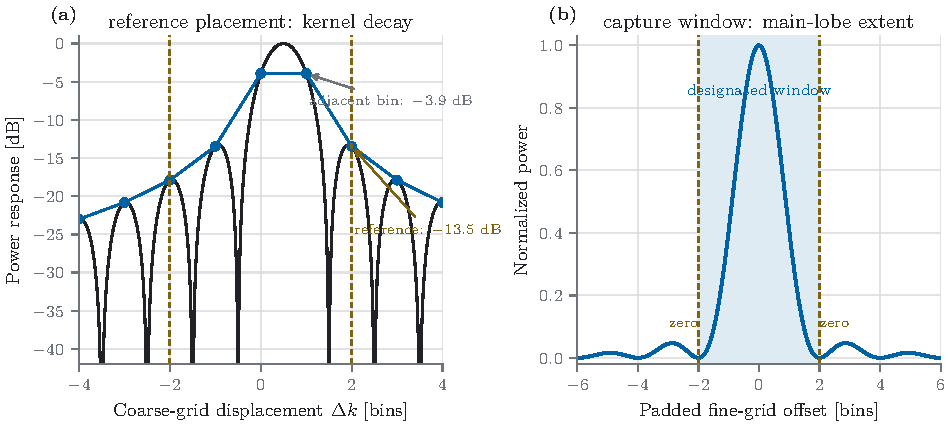
\includegraphics[width=0.98\linewidth]{figs/fig_dirichlet_duality.pdf}
\caption{The two $\pm 2$ displacements as dual applications of the Dirichlet response, Eq.~\eqref{eq:dirichlet}. (a) On the coarse grid, the references are placed at the kernel's decayed skirts: a tone at worst-case half-bin offset leaks $-3.9$~dB into the adjacent bin but only $-13.5$~dB at $\pm 2$, so the one-bin guard bounds self-contamination of the background estimate below $5\%$ in power (Section~\ref{sec:param:tradeoffs}). (b) On the padded fine grid, the window-axis kernel's main lobe spans exactly $\pm 2$ bins, so the designated detection window of Section~\ref{sec:pipeline:decision} is the main-lobe extent: an exclusion guard on one grid, a capture window on the other.}
\label{fig:dirichlet}
\end{figure}

\section{Target Profile Synthesis via DTV Pilot Matching}
\label{sec:param:target}

Section~\ref{sec:dtv:pilot} derived the detection beacon from first principles: a stationary, coherent pilot line at the exact rational offset $\tfrac{177}{572}$~MHz $\approx 309.440559$~kHz above each channel's lower allocation edge (Eq.~\eqref{eq:pilotfreq}; the implemented generator's hertz-rounded $309.441$~kHz, as noted there, is absorbed by the measured anchors). What remains is to map each of the $C = 23$ pilot frequencies --- UHF channels 14 through 36, on the raster of Section~\ref{sec:dtv:raster} --- into the receiver's channelized baseband and synthesize the matched filter.

The receiver's channelizer partitions the band into coarse channels of complex bandwidth $f_s$; pilot $c$ lands in a single coarse channel, and we define $\delta\!f_c = f_{\text{pilot}}^{(c)} - f_{\text{center}}^{(c)}$ as its baseband offset from that channel's center. The normalized tone frequency is
\begin{equation}
\nu_c = \frac{\delta\!f_c}{f_s} \pmod 1,
\end{equation}
under the receiver's baseband frame convention. Table~\ref{tab:channels} lists the complete mapping for the evaluated receiver. Two features of the table merit note. First, the offsets span $-190.6$ to $+184.4$~kHz --- nearly the full $\pm f_s/2$ --- because the 6~MHz broadcast raster and the $f_s = 390.625$~kHz channelizer raster are incommensurate, so successive pilots precess through the coarse-channel span. (Offsets are quoted in the RF frame; the detector's spectrally inverted baseband convention negates them, per the sign remark below.) The synthesized tone absorbs this entire channelization offset \emph{exactly}, which is what frees the fine spectral axis of Section~\ref{sec:pipeline:coherent} to resolve only residual transmitter error and slow drift within its $\pm 1.5$~kHz span. Second, the coarse-channel index \emph{decreases} as RF frequency increases, reflecting the receiver's spectrally inverted channel ordering; this inversion is absorbed entirely by the weight sign convention noted below.

\begin{table}[t]
\centering
\small
\caption{Pilot-to-channelizer mapping used by the evaluated configuration for the $C = 23$ monitored DTV channels: nominal pilot frequency, CHIME frequency-channel index (\texttt{freq\_id}, the identifier carried by all data products in this work), RF-frame baseband offset $\delta\!f_c = f_{\text{pilot}}^{(c)} - f_{\text{center}}^{(c)}$ of the pilot from the channel center, and resolved reference-placement status (Section~\ref{sec:param:refs}). Values are computed from the evaluated weight-generation configuration.}
\label{tab:channels}
\begin{tabular}{rrrrl}
\toprule
Ch. & Pilot (MHz) & \texttt{freq\_id} & $\delta\!f_c$ (kHz) & Placement \\
\midrule
14 & 470.309441 & 844 & $-3.059$ & edge-wrapped (lower) \\
15 & 476.309441 & 829 & $+137.566$ & nominal \\
16 & 482.309441 & 813 & $-112.434$ & nominal \\
17 & 488.309441 & 798 & $+28.191$ & nominal \\
18 & 494.309441 & 783 & $+168.816$ & nominal \\
19 & 500.309441 & 767 & $-81.184$ & nominal \\
20 & 506.309441 & 752 & $+59.441$ & nominal \\
21 & 512.309441 & 736 & $-190.559$ & nominal \\
22 & 518.309441 & 721 & $-49.934$ & nominal \\
23 & 524.309441 & 706 & $+90.691$ & nominal \\
24 & 530.309441 & 690 & $-159.309$ & nominal \\
25 & 536.309441 & 675 & $-18.684$ & nominal \\
26 & 542.309441 & 660 & $+121.941$ & nominal \\
27 & 548.309441 & 644 & $-128.059$ & nominal \\
28 & 554.309441 & 629 & $+12.566$ & nominal \\
29 & 560.309441 & 614 & $+153.191$ & nominal \\
30 & 566.309441 & 598 & $-96.809$ & nominal \\
31 & 572.309441 & 583 & $+43.816$ & nominal \\
32 & 578.309441 & 568 & $+184.441$ & nominal \\
33 & 584.309441 & 552 & $-65.559$ & nominal \\
34 & 590.309441 & 537 & $+75.066$ & nominal \\
35 & 596.309441 & 521 & $-174.934$ & nominal \\
36 & 602.309441 & 506 & $-34.309$ & nominal \\
\bottomrule
\end{tabular}
\end{table}

\textit{What the weights are.} The synthesis follows from one observation, and it is worth stating before the algebra because it explains every property the profile has. A single bin of a discrete Fourier transform,
\begin{equation}
\label{eq:dftbin}
X[\kappa] = \sum_{k=0}^{K-1} x[k] \, e^{-j 2\pi \kappa k / K},
\end{equation}
is an \emph{inner product} between the data and a sampled complex exponential. Computing a whole transform means computing $K$ of these against $K$ different exponentials, which is what an FFT accelerates. But the detector does not need a whole transform: the broadcast standard fixes the pilot frequency exactly (Eq.~\eqref{eq:pilotfreq}), so exactly one of those inner products carries the signal and the other $K-1$ are discarded work. Evaluating that one term directly is a single dot product of length $K$ --- and, because nothing forces the evaluation frequency onto the integer grid $\kappa/K$, it can be taken at the pilot's \emph{actual} normalized frequency $\nu_c$ rather than at the nearest bin. The weight profile is nothing more than that one DFT basis vector, conjugated and sampled at the tap index.

Three consequences follow immediately, and they are the reasons the architecture works. The cost is one multiply-accumulate chain per window rather than a transform, which is what fits the detector inside a small fraction of the real-time budget. The evaluation is off-grid, so the channelizer offset $\delta\!f_c$ of Table~\ref{tab:channels} is absorbed \emph{exactly} instead of leaving a scalloping loss --- and the fine axis downstream is then free to resolve only the residual transmitter error. And the basis vector is a compile-time constant: it depends on the standard and the receiver's raster, not on the data, so it can be quantized once, stored, hashed, and shared by every frame, which is what admits the exact integer datapath of Section~\ref{sec:impl:datapath}.

This also fixes the two-stage structure of the pipeline. The single-term DFT is applied to each $K$-tap window, collapsing it to one complex number; the $L = N/K = 128$ resulting numbers, one per window, are then transformed \emph{across} windows (Section~\ref{sec:pipeline:coherent}) to resolve frequency finely. The first transform is one fixed term at a known frequency; the second is a full, short transform over the unknown residual. Neither does the other's work.

Let $\mathbf{w}_{\text{target}}^{(c)} \in \mathbb{C}^{K \times 1}$ denote the primary target weight profile ($r = 0$) synthesized for the $c$-th DTV pilot. Written out, it is the conjugated basis vector of Eq.~\eqref{eq:dftbin} evaluated at $\nu_c$ and scaled to full fixed-point amplitude --- a complex sinusoidal matched filter tuned to the pilot carrier rotation across the $K = 128$ tap sub-frame duration:
\begin{equation}
\mathbf{w}_{\text{target}}^{(c)} = \begin{bmatrix}
w_{0,0}^{(c)} & w_{1,0}^{(c)} & \dots & w_{K-1,0}^{(c)}
\end{bmatrix}^T,
\qquad
w_{k,0}^{(c)} = \gamma \, \exp\left(j 2\pi \nu_c \, k\right), \quad k \in \{0, 1, \dots, K-1\}.
\end{equation}
Here $\gamma$ is the fixed-point full-scale amplitude: with $b$-bit signed components, $\gamma = 2^{b-1} - 1 = 7$ for the implemented \texttt{int4} representation. Driving every tap to full scale is the correct quantization policy for a constant-modulus profile --- it maximizes the ratio of signal power to quantization-noise power in the stored coefficients, since any smaller amplitude wastes representable range without changing the profile's shape; optimal loading of few-level quantizers is analyzed in detail for this receiver in \cite{menaparra2018}. The continuous-domain Euclidean norm is $\|\mathbf{w}_{\text{target}}^{(c)}\|_2 = \gamma \sqrt{K}$, i.e.\ a squared norm of $\gamma^2 K = 6272$; after component-wise rounding to the \texttt{int4} grid, the measured squared norms across the 23 configured channels fall in $[6280, 6418]$ --- scattered around the continuous value by up to $2.3\%$ because each channel's tone samples the quantization grid at different phases. The consequences of this scatter for the detection statistic's zero point are quantified in Section~\ref{sec:param:refs}. \textit{Remark on sign convention:} the implementation adopts the conjugate (negative-exponent) form of the tone, absorbing the receiver's spectrally inverted channel ordering visible in Table~\ref{tab:channels}; the coordinate convention is fixed \emph{per receiver profile} --- CHIME's second-Nyquist sampling inverts the baseband and orders \texttt{freq\_id} descending in RF, whereas a first-Nyquist receiver is upright and ascending --- and is recorded as explicit fields of the runtime bundle's detector contract (the conjugate tone form and the pre-kernel window time-reversal), detailed in Section~\ref{sec:impl:datapath}. Because a sense error mis-synthesizes the tone rather than mis-labelling it, it manifests as a complete detection miss; the acceptance gate is therefore an injected pilot at a known \emph{signed} offset, asserted to peak in the predicted bin, with the injector built from physical parameters independently of the detector's own convention path.

The reference profiles of Section~\ref{sec:param:refs} are the identical construction evaluated at neighboring frequencies: the same single-term DFT, displaced by $\pm \Delta k$ bins, which is why they share the target's norm structure and cancel against it in a ratio. By instantiating the detection pipeline across the $C = 23$ standardized pilot frequencies, the array evaluates 23 independent target weight profiles $\mathbf{w}_{\text{target}}^{(c)}$. Each target profile is accompanied by its own pair of frequency-shifted local reference profiles (nominally $\Delta k = \pm 2$ bins), as defined in Section~\ref{sec:param:refs}, yielding 23 distinct $K \times 3$ weight matrices $\mathbf{W}^{(c)}$.

\section{Reference Profile Generation via Unitary Shift}
\label{sec:param:refs}

To construct background reference profiles ($r \in \{1, 2\}$) that share identical structural characteristics with the target profile while satisfying the guard-band constraint of Section~\ref{sec:param:tradeoffs}, the target tone is displaced by a discrete frequency shift in the tap domain.

Let $\Delta k_r$ denote the resolved integer spectral bin displacement of reference $r$, nominally $\Delta k_1 = +2$ and $\Delta k_2 = -2$. The reference profile vectors are generated by point-wise complex phase rotation of the target profile:
\begin{equation}
w_{k, r} = w_{k, 0} \, \exp\left(j \frac{2\pi}{K} \Delta k_r \, k\right), \qquad k \in \{0, 1, \dots, K-1\}.
\end{equation}
In vector notation, let $\mathbf{E}(\Delta k) \in \mathbb{C}^{K \times K}$ define the diagonal phase-modulation matrix:
\begin{equation}
\mathbf{E}(\Delta k) = \text{diag}\left( 1, \, e^{j \frac{2\pi}{K} \Delta k}, \, e^{j \frac{2\pi}{K} \Delta k \cdot 2}, \, \dots, \, e^{j \frac{2\pi}{K} \Delta k (K-1)} \right),
\end{equation}
so that the complete weight matrix $\mathbf{W} \in \mathbb{C}^{K \times 3}$ is expressed compactly as:
\begin{equation}
\mathbf{W} = \begin{bmatrix}
\mathbf{w}_{\text{target}} & \mathbf{E}(\Delta k_1)\mathbf{w}_{\text{target}} & \mathbf{E}(\Delta k_2)\mathbf{w}_{\text{target}}
\end{bmatrix}.
\end{equation}
This construction has two properties worth making explicit. Structurally, each reference is the target's response displaced in frequency --- the same rectangular window, the same constant modulus, the same Dirichlet response of Eq.~\eqref{eq:dirichlet} recentered two bins away --- so the reference channels measure the background \emph{through the same instrument response} as the target channel measures the pilot, which is what makes their ratio a meaningful normalization. Algebraically, $\mathbf{E}(\Delta k)$ is unitary, so continuous-domain phase rotation preserves the Euclidean norm identically across all three columns ($\|\mathbf{w}_0\|_2 = \|\mathbf{w}_1\|_2 = \|\mathbf{w}_2\|_2$): in exact arithmetic the three channels have precisely equal gain, and the detection ratio's null center is exactly unity.

\textit{Adaptive placement.} The $\pm 2$-bin displacement is the nominal rule, not an invariant. Two per-channel hazards require resolution at weight-generation time. First, a nominal reference bin may fall outside the coarse channel's baseband span, in which case it wraps circularly within the channel (the projection is periodic in the tap domain, so the wrapped bin is the physically correct one); this is recorded as an \emph{edge-wrapped} placement. Second, a nominal reference bin may coincide with the channelizer's forbidden DC bin --- the bin onto which the receiver's DC offsets and quantizer bias concentrate after channelization, which therefore cannot serve as a background sample; in that case the reference is displaced outward bin-by-bin until clear (\emph{DC-shifted}), while a \emph{target} tone colliding with the DC bin is rejected outright rather than moved, since relocating the target would change what the detector measures. Every channel's resolved offsets, placement status, and warnings are recorded in the weight manifest and carried into the runtime calibration bundle, so the evaluated configuration is auditable after the fact. For the monitored array the resolution is almost entirely nominal: 22 of the 23 channels resolve at exactly $\pm 2$ bins, and the single exception is channel 14 (Table~\ref{tab:channels}), whose pilot lies only $+3.059$~kHz from the frame origin --- less than the $2$-bin displacement of $6.104$~kHz --- so its lower reference wraps across the channel edge. In implementation, each weight column is synthesized analytically at its \emph{resolved} normalized frequency and quantized independently, rather than by modulating the quantized target; the unitary-shift formalism above is the exact description of the continuous-domain construction, and quantization is applied once, at the end, to each column.

\textit{Quantized norms and the statistic's zero point.} Upon discretization to fixed-point \texttt{int4} representations, the three columns sample the quantization grid at different phase progressions, so their squared norms --- exact integers --- differ slightly. Across the 23 configured channels the measured norm-ratio factor $\mu_0 = 2\|\mathbf{w}_0\|^2 / (\|\mathbf{w}_1\|^2 + \|\mathbf{w}_2\|^2)$ falls in $[0.9853,\, 1.0111]$: the null center of the detection ratio is displaced from unity by up to $1.5\%$. This bias is not negligible: the coarse survey axis operates with thresholds within a fraction of a percent of unity (Section~\ref{sec:pipeline:decision}), and an uncorrected $1.5\%$ zero-point bias would exceed the available decision margin. The coarse recorded flag therefore applies $\mu_0$ as an \emph{exact rational} correction (the integer norms are known exactly, so the correction introduces no rounding); the fine CFAR rule of Section~\ref{sec:pipeline:decision} requires no correction at all, because the norm factor is common to every fine bin and cancels identically between the designated bins and the null-bulk baseline.

